%%%%
\section{Amostragem}

% http://maps.google.com/maps/ms?ie=UTF8&hl=en&msa=0&msid=116003586198857296821.00046d7e7367b947abe12&z=12

\begin{figure}[H]
\begin{center}
  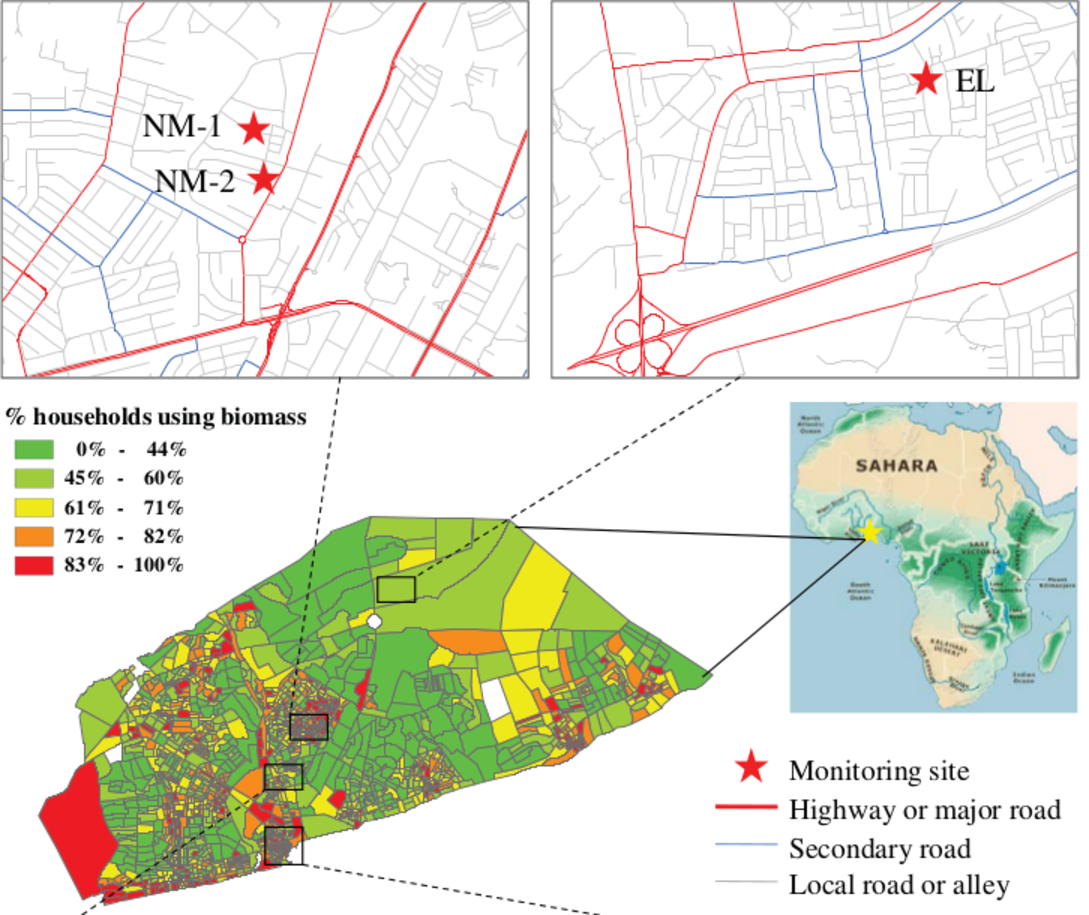
\includegraphics[width=0.6\textwidth]{../inputs/images/zheng/nima_mapa.pdf}
  \caption{Mapa de Nima. NM-1 ponto de amostragem na área residencial e 
           NM-2 ponto de amostragem na avenida. Porcentagem do uso da queima
           de biomassa para preparação de alimentos em residências usando dados
           do censo de 2000 \citep{ghanacensus2003} \label{fig:nima_mapa}}
\end{center}
\end{figure}

A localização geográfica dos dois pontos de medição, distantes entre si 330
metros, é apresentada na figura
\ref{fig:nima_mapa}, sendo NM-1 na rua \textit{Sam Road}, quarteirão residencial,
e NM-2 na \textit{Nima Road}, via arterial de 2,8 km na direção norte-sul, 
direciona o tráfego de pequenas vias locais para o centro, atravessando áreas de 
comércio variado. 
%distante 5 km do aeroporto de Acra

As medições ocorreram entre 11 de novembro de 2006 e 15 de agosto de 2008 com 
amostragem de 48 horas de duração. Falta de eletricidade, problemas com 
amostrador, filtros danificados ou contaminado na manipulação e ausência do 
operador nas trocas foram as principais ocorrências encotradas. 

As amostras foram coletadas em filtro de Teflon do tipo \textbf{PTFE} 
com diâmetro de 37 mm e orifícios com raio de 0,1 $\mu m$. A área de deposição 
nos filtros foi de 7,32 $\pm$ 0,36 $cm^2$.

Impactadores são equipamentos responsáveis pela coleta e separação das 
partículas baseando-se na inércia. Utilizou-se impactador tipo Harvard, 
descrito por \citet{marple1987}, com $D_{50}$ de $10 \mu m$ e fluxo de 
$10,0 L/min$ para coleta de $MP_{10}$. Para $MP_{2,5}$, foi instalado 
outro impactador pararelo, também do tipo Harvard, mas com $D_{50}$ de 
$2,5 \mu m$ acoplado com um \textit{inlet} responsável fazer a filtragem de 
somentes partículas com diâmetros aerodinâmicos menores que 2,5 $\mu m$. 
Os volumes foram estimados por um integrador/totalizador de volume.

Filtros brancos de campo e laboratórios foram separados para avaliar 
possíveis contaminações de fábrica ou de manipulação das amostras. 
Os filtros foram pesados no laboratório da HSPH em balança 
microanalítica (Mettler Toledo MT5) com precisão de $\pm 1 \mu g$, 
seguindo procedimentos padrões de controle de umidade ($39 \pm 2 \%$), 
temperatura ($20,5 \pm 0,2 ^{\circ} C$) e eliminação de cargas eletrostáticas 
com fonte de polônio. 
Cada medida de pesagem foi realizada duas vezes, sendo a média o valor 
final considerado.
